\documentclass[aspectratio=169,11pt]{beamer}
\usepackage{fathomnet-course}
% generated by write_numbers.py from results/reference_results.json - do not edit
\newcommand{\RefCrops}{23{,}664}
\newcommand{\RefDives}{1{,}465}
\newcommand{\RefTopTenDives}{21\,\%}
\newcommand{\RefTwoTrain}{444}
\newcommand{\RefTwoTest}{148}
\newcommand{\RefThr}{0.05}
\newcommand{\RefThrTrain}{98.4\,\%}
\newcommand{\RefThrTest}{98.0\,\%}
\newcommand{\RefCSPhylumMajority}{30.4\,\%}
\newcommand{\RefCSPhylumCentroid}{26.4\,\%}
\newcommand{\RefCSPhylumKnn}{55.0\,\%}
\newcommand{\RefCSPhylumTree}{50.3\,\%}
\newcommand{\RefCSLabelMajority}{1.3\,\%}
\newcommand{\RefCSLabelCentroid}{15.9\,\%}
\newcommand{\RefCSLabelKnn}{33.6\,\%}
\newcommand{\RefCSLabelTree}{23.7\,\%}
\newcommand{\RefCSLabelBest}{33.6\,\%}
\newcommand{\RefZooBestName}{neural network (MLP)}
\newcommand{\RefZooBest}{64.6\,\%}
\newcommand{\RefZooBestPixels}{46.3\,\%}
\newcommand{\RefZooBestColour}{48.4\,\%}
\newcommand{\RefZooRows}{majority baseline & 1.3\,\% & 1.3\,\% & $<$1\,s \\
nearest centroid & 39.9\,\% & 37.9\,\% & 2\,s \\
5-nearest neighbours & 69.9\,\% & 53.4\,\% & $<$1\,s \\
decision tree & 100.0\,\% & 20.5\,\% & 48\,s \\
random forest & 100.0\,\% & 56.1\,\% & 93\,s \\
logistic regression & 90.7\,\% & 63.7\,\% & 21\,s \\
neural network (MLP) & 92.4\,\% & 64.6\,\% & 13\,s \\}
\newcommand{\RefRandomAcc}{63.5\,\%}
\newcommand{\RefRandomAccKnn}{53.5\,\%}
\newcommand{\RefTrainLogregRandom}{90.7\,\%}
\newcommand{\RefTrainKnnRandom}{70.0\,\%}
\newcommand{\RefImageAcc}{57.5\,\%}
\newcommand{\RefImageAccKnn}{45.5\,\%}
\newcommand{\RefTrainLogregImage}{91.1\,\%}
\newcommand{\RefTrainKnnImage}{71.0\,\%}
\newcommand{\RefDiveAcc}{49.6\,\%}
\newcommand{\RefDiveAccKnn}{35.5\,\%}
\newcommand{\RefTrainLogregDive}{91.0\,\%}
\newcommand{\RefTrainKnnDive}{71.6\,\%}
\newcommand{\RefSeenDiveRandom}{97\,\%}
\newcommand{\RefRecallRows}{species & 33 & 67\,\% \\
genus & 21 & 69\,\% \\
family & 8 & 64\,\% \\
order & 6 & 56\,\% \\
class & 6 & 44\,\% \\
phylum & 1 & 27\,\% \\
other rank & 4 & 58\,\% \\}
\newcommand{\RefSevKingdom}{55\,\%}
\newcommand{\RefSevNear}{21\,\%}
\newcommand{\RefRandPhylumAcc}{80.0\,\%}
\newcommand{\RefDivePhylumAcc}{72.6\,\%}
\newcommand{\RefDiveFone}{0.475}
\newcommand{\RefDiveAccSingle}{49.8\,\%}

\title{Testing honestly}
\subtitle{\coursetitle\\[2pt]\small Session 4 -- reading results, judging mistakes, new expeditions}
\date{}
\author{}
\begin{document}
\maketitle

\begin{frame}{Where we are}
CNN features + logistic regression, 79 labels, random split: \hl{\RefRandomAcc} of the test crops correct.\\[8pt]
Today, three questions a biologist must ask before using it:
\begin{enumerate}
  \item \textbf{Which} labels does it get wrong -- and which does it confuse?
  \item How \textbf{biologically} wrong are the mistakes?
  \item Would it work on a \textbf{new expedition}?
\end{enumerate}
\end{frame}

\section{Reading results}

\begin{frame}{Accuracy, recall, precision}
\begin{columns}[T]
\column{0.5\textwidth}
\small
For one label, e.g.\ \emph{Asteroidea}:
\begin{description}[Precision]
\item[Recall] of all true sea stars, which fraction did the classifier \emph{find}?
\item[Precision] of all crops it \emph{called} sea star, which fraction really are?
\item[F1] combines both: $\frac{2\cdot P\cdot R}{P+R}$
\end{description}
Over all labels:
\begin{description}[Balanced acc.]
\item[Accuracy] fraction of all crops correct
\item[Balanced acc.] mean recall over labels
\item[Macro-F1] mean F1 over labels
\end{description}
\column{0.46\textwidth}
\begin{alertblock}{Why more than accuracy?}
A survey video: 900 brittle stars, 100 sea pens.\\
``Always say brittle star'' $\Rightarrow$ accuracy \textbf{90\,\%}, but balanced accuracy only \textbf{50\,\%} -- it never finds a single sea pen.
\end{alertblock}
\small In our data every label has $\approx$300 crops, so the numbers are close. In real surveys they are not.
\end{columns}
\end{frame}

\begin{frame}{The confusion matrix}
\begin{columns}[c]
\column{0.45\textwidth}
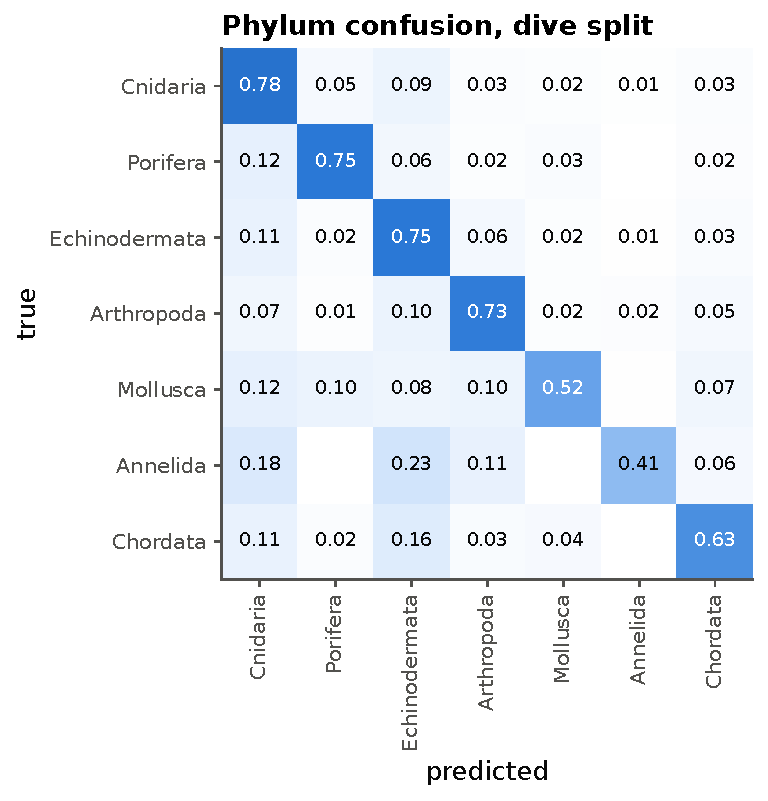
\includegraphics[width=\linewidth]{figures/confusion_phylum.pdf}
\column{0.52\textwidth}
\small
\begin{itemize}
  \item rows: the \textbf{true} phylum; columns: the \textbf{predicted} phylum (both derived from the 79-label prediction)
  \item each row sums to 1; diagonal = recall
  \item off-diagonal = which groups are mixed up
\end{itemize}
\muted{\scriptsize CNN + logistic regression, tested on dives not seen in training}\\[6pt]
\task{\small Find the largest off-diagonal cell. Can you explain it biologically (shape, colour, habitat, both sessile)?}
\end{columns}
\end{frame}

\begin{frame}{Which labels are hard?}
\begin{columns}[c]
\column{0.5\textwidth}
\small
\textbf{Recall by the rank of the label} (random split):\\[4pt]
\begin{tabular}{@{}lrr@{}}
\toprule
label is a \dots & labels & mean recall \\
\midrule
\RefRecallRows
\bottomrule
\end{tabular}
\column{0.46\textwidth}
\small
Labels at \hl{coarse ranks} (class, order, family) are harder: a class label like \emph{Asteroidea} covers hundreds of very different-looking species -- and is used exactly when the animal is \emph{hard to see}.\\[6pt]
\muted{Also hard: tiny and blurry crops, labels that look like their relatives.}
\end{columns}
\end{frame}

\section{Biologically wrong}

\begin{frame}{Not all mistakes are equal}
\begin{columns}[c]
\column{0.5\textwidth}
\small
\begin{tabular}{@{}llll@{}}
\toprule
truth & prediction & agree up to & \\
\midrule
\emph{Sebastes} & \emph{S.\ diploproa} & genus & mild \\
Asteroidea & Ophiuroidea & phylum & medium \\
Asteroidea & Actiniaria & kingdom & severe \\
\bottomrule
\end{tabular}\\[8pt]
The FathomNet 2025 score counts the steps through the tree of life between truth and prediction (0--12).
\column{0.47\textwidth}
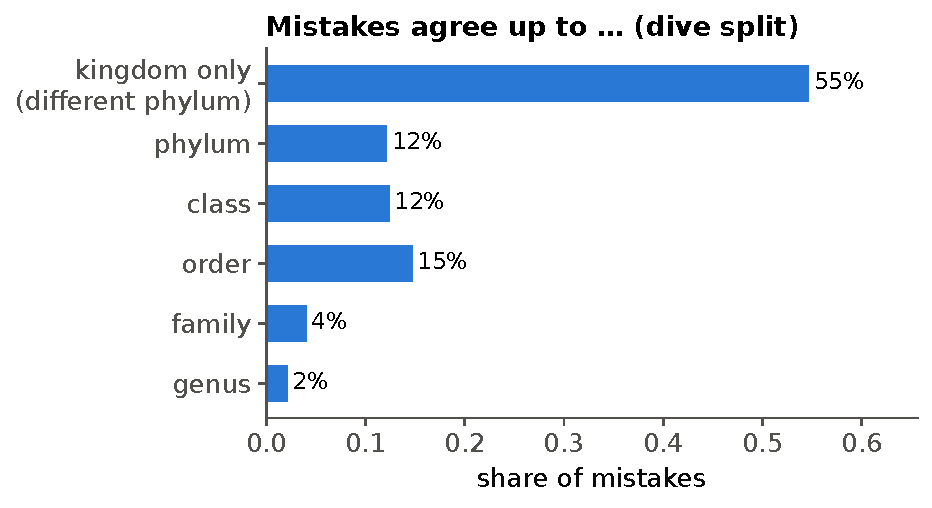
\includegraphics[width=\linewidth]{figures/mistake_severity.pdf}
\end{columns}
\vspace{2pt}
\small On new dives, \hl{\RefSevKingdom} of the mistakes do not even get the phylum right; only \RefSevNear\ are near misses (same order, family or genus).
\end{frame}

\begin{frame}{Asking for a coarser rank}
\begin{columns}[c]
\column{0.55\textwidth}
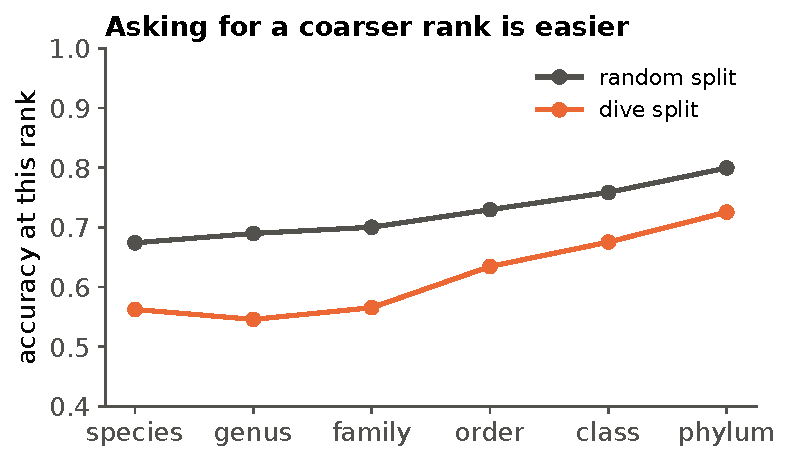
\includegraphics[width=\linewidth]{figures/accuracy_by_rank.pdf}
\column{0.42\textwidth}
\small
We keep the 79-label prediction but only check whether its \emph{phylum}, \emph{class}, \dots\ is right.\\[4pt]
Phylum correct: \RefRandPhylumAcc\ (random split), \RefDivePhylumAcc\ (new dives).\\[6pt]
\muted{For a survey this suggests: report at the rank where the classifier is reliable, and let experts check the rest.}
\end{columns}
\end{frame}

\section{New expeditions}

\begin{frame}{The trap: frames from the same dive}
\begin{columns}[c]
\column{0.5\textwidth}
\small
\begin{itemize}
  \item \RefCrops\ crops come from only \RefDives\ dives; the 10 largest dives contribute \RefTopTenDives\ of all crops.
  \item Frames of one dive share site, light, camera -- and often \textbf{the same individual}.
  \item A \emph{random} split puts near-identical crops in train \emph{and} test: \RefSeenDiveRandom\ of the test crops come from a dive that is also in training.
\end{itemize}
\column{0.46\textwidth}
\begin{block}{Three ways to split}
\small
\textbf{random}: crop by crop\\
\textbf{image}: all crops of one video frame together\\
\textbf{dive}: all crops of one dive together $\Rightarrow$ the test set is a \hl{new expedition}
\end{block}
\end{columns}
\end{frame}

\begin{frame}{The result}
\begin{columns}[c]
\column{0.56\textwidth}
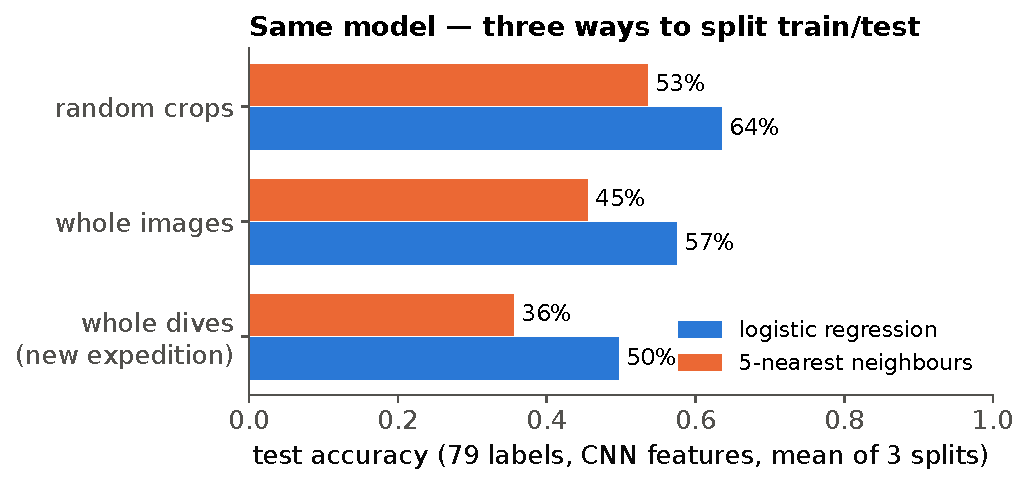
\includegraphics[width=\linewidth]{figures/split_comparison.pdf}
\column{0.41\textwidth}
\small
Same features, same classifier: accuracy falls from \hl{\RefRandomAcc} to \hl{\RefDiveAcc} when the test animals come from dives the classifier has never seen.\\[6pt]
The prize-winning models of FathomNet 2025 show the same: 98\,\% on known images, 57--61\,\% on new dives.\\[6pt]
\textbf{Report the dive-split number.} It is the honest estimate for the next cruise.
\end{columns}
\end{frame}

\begin{frame}{Checklist before you trust a classifier}
\begin{enumerate}
  \item Was it tested on data it has \textbf{never seen} -- including new sites, dives, cameras?
  \item Is the result \textbf{better than the baseline}?
  \item Which labels are weak (per-label recall)? Are \emph{your} species among them?
  \item Are the mistakes \textbf{near misses} or far off? At which rank is it reliable?
  \item Are rare labels and imbalanced classes reported fairly (balanced accuracy, macro-F1)?
  \item Has someone \textbf{looked at the mistakes}? Some ``mistakes'' are wrong labels.
\end{enumerate}
\end{frame}

\begin{frame}{Lab 3 -- testing honestly}
\task{
\begin{enumerate}
  \item Compute accuracy, balanced accuracy and macro-F1. Explain the difference.
  \item Find the 10 hardest labels. Do coarse-rank labels do worse?
  \item Confusion matrix by phylum and within your phylum: which pairs are confused, and why?
  \item Mistake severity: near or far misses?
  \item Random vs.\ image vs.\ dive split: measure the drop and explain it.
  \item Look at the most confident mistakes: classifier error, bad crop, or wrong label?
\end{enumerate}}
\end{frame}
\end{document}
